\section{Numerical steepest descent}
\label{Sec4:NumericalSteepestDecent}
Consider first the one-dimensional case of the oscillatory integral in~\Cref{Eq4:oscillatoryIntegral}. To illustrate the technique of numerical steepest descent we consider the integral
\begin{equation}\label{Eq:NSD1Dlinear}
	I = \int_a^b f(x) \euler^{\imag \omega g(x)}\idiff x.
\end{equation}
This integral is highly oscillatory for large values of $\omega$ and non-constant oscillator $g$ due to the exponential factor $\euler^{\imag \omega g(x)}$. However, this factor is not oscillatory along paths $z=h_x(p)$ (parameterized with the parameter $p$) in the complex plane satisfying
\begin{equation}\label{Eq4:gh_xp}
	g(h_x(p)) = \imag p + g(x)
\end{equation}
This is because, for a given $x$ we have $\euler^{\imag \omega g(z)}=\euler^{-\omega p}\euler^{\imag \omega g(x)}$, and the factor $\euler^{-\omega p}$ is not oscillatory. In fact, it is exponentially decaying in the complex plane. The idea of numerical steepest descent is to evaluate the oscillatory integral along such paths in the complex plane. For the case of no stationary points where $g'(z)=0$ Theorem 2.1 in~\cite{Huybrechs2007tco} states that the integral in~\Cref{Eq:NSD1Dlinear} may be decomposed as
\begin{equation*}
	I = F(a)-F(b) + \bigoh(\euler^{-\omega d_0})
\end{equation*}
where (with the substitution $p=q/\omega$)
\begin{align}\label{Eq4:F_j}
	F(\xi) &= \int_0^\infty f(h_{\xi}(p))\euler^{\imag\omega(g(\xi)+\imag p)} h_{\xi}'(p)\idiff p\\
	&= \frac{\euler^{\imag\omega g(\xi)}}{\omega}\int_0^\infty f(h_{\xi}(q/\omega))\euler^{-q} h_{\xi}'(q/\omega)\idiff q.
\end{align}
Consider now stationary points $z=\xi$ of order $r$ (that is, $g'(\xi)=g''(\xi)=\dots=g^{(r)}(\xi) = 0$ and $g^{(r+1)}(\xi)\not=0$). Since the inverse of $g$ is multivalued around these points, several paths $h_{\xi,j}$, $j=0,\dots,r$, exists that all satisfy~\Cref{Eq4:gh_xp}. Using a Taylor expansion of $g(z)$ around $z=\xi$ yields
\begin{equation*}
	h_{\xi,j}(p) \sim \xi + \sqrt[r+1]{\imag\frac{(r+1)!p}{g^{(r+1)}(\xi)}},\qquad h_{\xi,j}'(p) \sim \frac{1}{r+1}\sqrt[r+1]{\imag\frac{(r+1)!}{g^{(r+1)}(\xi)}}p^{\frac{1}{r+1}-1}.
\end{equation*}
That is if we have a stationary point at $z=\xi$ of order $r$ the substitution introduces weakly singular behavior near the real axis. This can be handled by a generalized Gauss Laguerre quadrature as explained in~\cite{Huybrechs2007tco}.

Alternatively, Freud-type Gaussian (GF) quadrature may be applied. With an additional substitution $q=u^{r+1}$ we get
\begin{equation}\label{Eq4:dh_xi}
	h_{\xi,j}(p) \sim \xi + \sqrt[r+1]{\imag\frac{(r+1)!}{\omega g^{(r+1)}(\xi)}} u,\qquad h_{\xi,j}'(p) \sim \frac{\omega}{r+1}\sqrt[r+1]{\imag\frac{(r+1)!}{\omega g^{(r+1)}(\xi)}}u^{-r}
\end{equation}
since $\diff q = (r+1)u^r \diff u$ the function $F_j(\xi)$ in~\Cref{Eq4:F_j} may be written as
\begin{align*}
	F_j(\xi) &= \frac{(r+1)\euler^{\imag\omega g(\xi)}}{\omega}\int_0^\infty f(h_{\xi,j}(u^{r+1}/\omega))\euler^{-u^{r+1}} h_{\xi,j}'(u^{r+1}/\omega)u^r\idiff u.
\end{align*}
The factor $u^r$ effectively cancels the singular behavior of $h_{\xi,j}'(p)$ in~\Cref{Eq4:dh_xi}.

For the case $f(x) = x^n$ and $g(x)=x^m$, the integral in~\Cref{Eq:NSD1Dlinear} can be expressed in terms of the (upper) incomplete gamma function (for integer $m$)
\begin{equation*}
	\int_0^1 x^n \euler^{\imag \omega x^m}\idiff x = \frac{1}{m(-\imag\omega)^{\frac{n+1}{m}}}\left[\Gamma\left(\frac{n+1}{m},0\right)-\Gamma\left(\frac{n+1}{m},-\imag\omega\right)\right]
\end{equation*}
where
\begin{equation*}
	\Gamma(s,z) = \int_z^\infty t^{s-1}\euler^{-t}\idiff t
\end{equation*}
is implemented in \MATLAB as \verb|igamma(s,z)|. For integer $n$ and $m=1$ we have
\begin{equation*}
	\Gamma(n+1,z) = \euler^{-z}\sum_{m=0}^n\frac{n!}{m!}z^m
\end{equation*}
such that
\begin{equation*}
	\int_0^1 x^n \euler^{\imag \omega x}\idiff x = \frac{1}{(-\imag \omega)^{n+1}}\left[n! -  \euler^{\imag \omega}\sum_{m=0}^n \frac{n!}{m!}(-\imag \omega)^m\right].
\end{equation*}
With $g(z) = z$ we have the two paths $h_0(p) = \imag p$ and $h_1(p) = \imag p+1$ starting from $z=0$ and $z=1$, respectively. Along these paths we have $z=h_x(p)$ and $\diff z=h_x'(p)\idiff p=\imag\idiff p$. Such that the integral in~\Cref{Eq:NSD1Dlinear} may be decomposed as
\begin{align*}
	I_1 &= \int_0^1 x^n \euler^{\imag \omega x}\idiff x \\
	  &= \euler^{\imag\omega g(0)}\int_0^\infty f(h_0(p))\euler^{-\omega p}h_0'(p)\idiff p - \euler^{\imag\omega g(1)}\int_0^\infty f(h_1(p))\euler^{-\omega p}h_1'(p)\idiff p\\
	  &= \int_0^\infty \imag(\imag p)^n\euler^{-\omega p}\idiff p - \euler^{\imag\omega}\int_0^\infty \imag(\imag p+1)^n\euler^{-\omega p}\idiff p\\
	  &= \frac{\imag}{\omega}\left[\int_0^\infty (\imag q/\omega)^n\euler^{-q}\idiff q - \euler^{\imag\omega}\int_0^\infty (\imag q/\omega+1)^n\euler^{-q}\idiff q\right].
\end{align*}
The generalized Gauss-Laguerre (GGL) quadrature rule integrates the integral
\begin{equation*}
	\int_0^\infty \tilde{f}(q)x^\alpha\euler^{-q}\idiff q,\quad \alpha = -\frac{r}{r+1}
\end{equation*}
exactly for polynomials $\tilde{f}(q)$ of order up to $2n_{\mathrm{qp}}-1$, and so we should expect exact results whenever $n\leq 2n_{\mathrm{qp}}-1$. This is indeed observed in~\Cref{Fig4:tasks_1}.
\begin{figure}
	\centering
	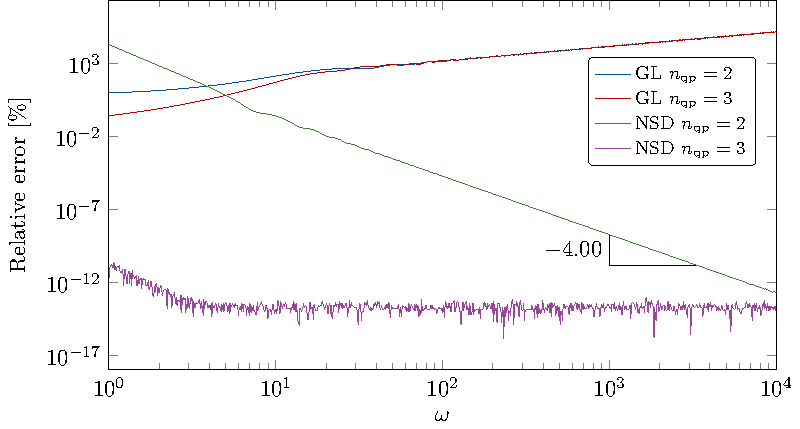
\includegraphics{tasks_1}
	\caption{\textbf{Numerical steepest descent}: The relative numerical error of the NSD and Gauss Legendre quadrature applied to the integral $I_1$ with $n=5$. Machine epsilon results is expected for the NSD when using $n_{\mathrm{qp}}=3$. Correct convergence rate of $-2n_{\mathrm{qp}}-\alpha=-4$ is observed when using $n_{\mathrm{qp}}=2$ (note that $\alpha=0$ for $I_1$).}
	\label{Fig4:tasks_1}
\end{figure}

Consider now the case $m=2$. The paths are then given by $h_x(p) = \pm\sqrt{\imag p + x^2}$. For the point $x=1$ the sign must be chosen to satisfy $h_1(0) = 1$. Thus, the path starting from $z=1$ is given by $h_1(p) = \sqrt{\imag p + 1}$. For the point $x=0$ each of the signs satisfy $h_0(0) = 0$, and must be chosen such that this paths share the same branch as the path from $x=1$. Hence, the path starting from $z=0$ is given by $h_0(p) = \sqrt{\imag p}$. In~\Cref{Fig4:paths} these paths are visualized on top of a contour plot of $\Im(\imag g(z)) = (\Re z)^2-(\Im z)^2$.
\begin{figure}
	\centering
	\includegraphics{contourplot_1}
	\caption{\textbf{Numerical steepest descent}: Paths in the complex plane at which the imaginary part of the oscillator $g(z)$ is constant. The paths from $z=0$ and $z=1$ are drawn as red dashed lines, with $n_{\mathrm{qp}}=5$ Gauss Laguerre quadrature points on top. Note that due to the scaling $q=\omega p$ the quadrature points will get closer to the real axis as $\omega$ gets smaller (here, $\omega=10$).}
	\label{Fig4:paths}
\end{figure}
Along these two paths we have $z=h_x(p)$ and $\diff z=h_x'(p)\idiff p=\imag/2(\imag p+x^2)^{-1/2}\idiff p$. Such that the integral in~\Cref{Eq:NSD1Dlinear} may be decomposed as
\begin{align*}
	I_2 &= \int_0^1 x^n \euler^{\imag \omega x^2}\idiff x \\
	  &= \euler^{\imag\omega g(0)}\int_0^\infty f(h_0(p))\euler^{-\omega p}h_0'(p)\idiff p - \euler^{\imag\omega g(1)}\int_0^\infty f(h_1(p))\euler^{-\omega p}h_1'(p)\idiff p\\
	  &= \int_0^\infty \frac{\imag}{2}(\imag p)^{n/2-1/2}\euler^{-\omega p}\idiff p - \euler^{\imag\omega}\int_0^\infty \frac{\imag}{2}(\imag p+1)^{n/2-1/2}\euler^{-\omega p}\idiff p\\
	  &= \frac{\imag}{2\omega}\left[\int_0^\infty (\imag q/\omega)^{n/2-1/2}\euler^{-q}\idiff q - \euler^{\imag\omega}\int_0^\infty (\imag q/\omega+1)^{n/2-1/2}\euler^{-q}\idiff q\right]\\
	  &= \left[\int_0^\infty (\imag u/\omega)^n\euler^{-u^2}\idiff u - \frac{\imag\euler^{\imag\omega}}{\omega}\int_0^\infty u(\imag u^2/\omega+1)^{n/2-1/2}\euler^{-u^2}\idiff u\right].
\end{align*}
In~\Cref{Fig4:tasks_2} we can again observe convergence rates close to the expected values. The GGL quadrature and GF quadrature perform very similar here. A heuristic study was made on these two quadrature techniques and the performance depend on the oscillator function $g$. For the oscillators with stationary points of high order, the GF points seems to be desirable, but for low $r$ the GLL points gave the best results. Further investigation into this is suggested as future work.
\begin{figure}
	\centering
	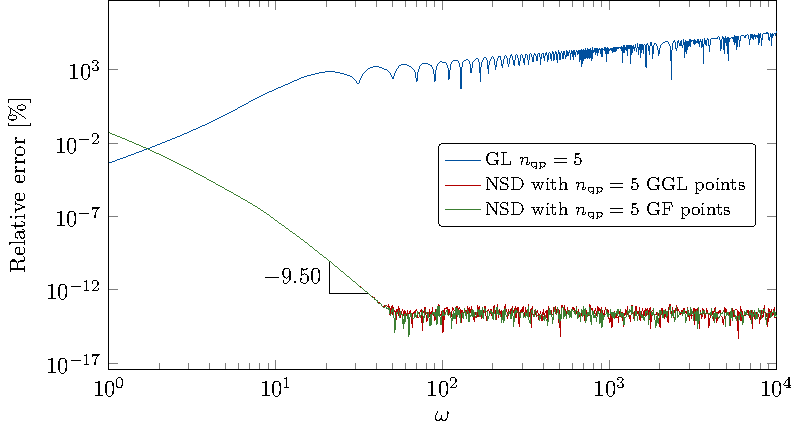
\includegraphics{tasks_2}
	\caption{\textbf{Numerical steepest descent}: The relative numerical error of the NSD and Gauss Legendre quadrature applied to the integral $I_2$ with $n=4$. Correct convergence rate of $-2n_{\mathrm{qp}}-\alpha=-9.5$ is observed when using $n_{\mathrm{qp}}=5$ (note that $\alpha=-0.5$ for the path starting from $z=0$ and that $\alpha=0$ for the path starting from $z=1$ such that GGL points and GF points are identical on this path).}
	\label{Fig4:tasks_2}
\end{figure}

\subsection{Starting value for Newton iterations}
We use Taylor expansion around $\xi$ to find a starting value for Newton iterations to obtain the path $h_\xi(p)$
\begin{equation*}
	g(x) = g(\xi) + g'(\xi)(x-\xi) + \frac{1}{2}g''(\xi)(x-\xi)^2 + \dots
\end{equation*}
where $x=h_\xi(p)$. Since 
\begin{equation}\label{Eq4:path}
	g(h_\xi(p)) = g(\xi)+\imag p
\end{equation}
we get
\begin{equation*}
	\imag p = g'(\xi)(h_\xi(p)-\xi) + \frac{1}{2}g''(\xi)(h_\xi(p)-\xi)^2 + \dots
\end{equation*}
So in case of a stationary point of order $r$ we can use
\begin{align*}
	h_\xi(p) &\approx \xi + \euler^{\frac{2\PI j\imag}{r+1}}\sqrt[r+1]{\frac{(r+1)!p}{g^{(r+1)}(\xi)}\imag} \\
	&= \xi + \exp\left[\frac{(4j+1)\PI  - 2\arg{g^{(r+1)}(\xi)}}{2(r+1)}\imag\right]\sqrt[r+1]{\frac{(r+1)!p}{|g^{(r+1)}(\xi)|}}.
\end{align*}
where $j=0,1,\cdots,r$ must be chosen such that the endpoints of to neighboring paths have the same sign of the imaginary part.

Whenever $g'(\xi)\not=0$ and $g''(\xi)=0$ we simply use the linear approximation
\begin{equation*}
	h_\xi(p) \approx \xi + \frac{\imag p}{g'(\xi)}.
\end{equation*}
If $g'(\xi)\not=0$ and $g''(\xi)\neq 0$, we use a quadratic approximation
\begin{equation*}
	h_\xi(p) \approx \xi + \frac{-g'(\xi)\pm \sqrt{g'(\xi)^2+2\imag g''(\xi)p}}{g''(\xi)}
\end{equation*}
The sign can be determined (using \Cref{Eq4:path}) by the following requirement
\begin{equation}\label{Eq4:condh_xi}
	h_\xi'(p) = \frac{\imag}{g'(h_\xi(p))}\qquad \Rightarrow\qquad h_\xi'(0)= \frac{\imag}{g'(h_\xi(0))}= \frac{\imag}{g'(\xi)}
\end{equation}
such that (since $z=\sgn{\Re{z}}\sqrt{z^2}$)
\begin{equation*}
	h_\xi(p) \approx \xi - \frac{g'(\xi)-\sgn{\Re{g'(\xi)}}\sqrt{g'(\xi)^2+2\imag g''(\xi)p}}{g''(\xi)}.
\end{equation*}
Slightly more involved formulas can be obtained for the cubic approximation (requiring $g^{(3)}(\xi)\neq 0$)
\begin{equation*}
	h_\xi(p) \approx \xi + W -\frac{P}{3W}-\frac{g''(\xi)}{g^{(3)}(\xi)},\quad W = \euler^{2\PI\imag j/3}\left(\frac{Q}{2}+\sqrt{\frac{Q^2}{4}+\frac{P^3}{27}}\right)^{1/3},\quad j=0,1,2
\end{equation*}
where
\begin{equation*}
	P = \frac{6g'(\xi)}{g^{(3)}(\xi)} - 3\left[\frac{g''(\xi)}{g^{(3)}(\xi)}\right]^2,\qquad Q = \frac{6g'(\xi)g''(\xi)}{\left[g^{(3)}(\xi)\right]^2}+\frac{6\imag p}{g^{(3)}(\xi)} - 2\left[\frac{g''(\xi)}{g^{(3)}(\xi)}\right]^3.
\end{equation*}
The integer $j$ must be determined from \Cref{Eq4:condh_xi}. 

Alternatively, a Taylor expansion can be obtained by expanding $h_\xi(p)$ around $p=0$
\begin{equation*}
	h_\xi(p) = \xi + h'_\xi(0)p + \frac12h''_\xi(0)p^2 + \frac{1}{6}h^{(3)}_\xi(0)p^3 + \frac{1}{24}h^{(4)}_\xi(0)p^4+\dots
\end{equation*}
where one can compute 
\begin{align*}
	h'_\xi(0) &= \frac{\imag}{g'(\xi)},\quad h''_\xi(0) = \frac{g''(\xi)}{\left[g'(\xi)\right]^3},\quad h^{(3)}_\xi(0) = \frac{g^{(3)}(\xi)g'(\xi)-3\left[g''(\xi)\right]^2}{\left[g'(\xi)\right]^5}\imag\\
	h^{(4)}_\xi(0) &= -\frac{g^{(4)}(\xi)\left[g'(\xi)\right]^2-10g^{(3)}(\xi)g''(\xi)g'(\xi)+15\left[g''(\xi)\right]^3}{\left[g'(\xi)\right]^7}                                                                                                                                                                                                                                                                                         
\end{align*}
with the assumption that $g'(\xi)\not=0$. Because of this assumption, this expansion cannot be used to approximate paths from stationary points.

\subsection{The case of no critical points or resonance points in 2D}
Assuming we first integrate in the $\eta$-direction, we define the path $v_\eta(\xi,q)$ in the complex plane defined by
\begin{equation*}
	g(\xi,v_{\eta_j}(\xi,q))=g(\xi,\eta_j)+\imag q
\end{equation*}
such that
\begin{align*}
	I &= \int_{\xi_1}^{\xi_n}\int_{\eta_1}^{\eta_m} f(\xi,\eta)\euler^{\imag k g(\xi,\eta)}\idiff\eta\idiff \xi\\
	&=\int_{\xi_1}^{\xi_n}\left[\euler^{\imag k g(\xi,\eta_1)}\int_0^\infty f(\xi,v_{\eta_1}(\xi,q))\euler^{-k q}\pderiv{v_{\eta_1}}{q}(\xi,q)\idiff q\right.\\
	&{\hskip4em\relax}\left. -\euler^{\imag k g(\xi,\eta_m)}\int_0^\infty f(\xi,v_{\eta_m}(\xi,q))\euler^{-k q}\pderiv{v_{\eta_m}}{q}(\xi,q)\idiff q\right]\idiff \xi
\end{align*}
We continue by defining
\begin{equation*}
	g(u_{\xi_i}(p),\eta_j)=g(\xi_i,\eta_j)+\imag p
\end{equation*}
such that
\begin{equation*}
	I = F_{\mathrm{yx}}(\xi_1,\eta_1) - F_{\mathrm{yx}}(\xi_2,\eta_1) - \left[F_{\mathrm{yx}}(\xi_1,\eta_2)-F_{\mathrm{yx}}(\xi_2,\eta_2)\right]
\end{equation*}
where
\begin{equation}\label{Eq4:F_yx}
\begin{aligned}
	F_{\mathrm{yx}}(\xi,\eta) = \euler^{\imag k g(\xi,\eta)}\int_0^\infty\int_0^\infty &f(u_\xi(p),v_{\eta}(u_{\xi}(p),q))\euler^{-k (q+p)}\\
	&{\hskip1em\relax}\cdot\pderiv{v_\eta}{q}(u_{\xi}(p),q)u_\xi'(p)\idiff q\idiff p.
\end{aligned}
\end{equation}
Similar expressions may be found by first integration over the $\xi$-direction
\begin{equation*}
	I = F_{\mathrm{xy}}(\xi_1,\eta_1) - F_{\mathrm{xy}}(\xi_2,\eta_1) - \left[F_{\mathrm{xy}}(\xi_1,\eta_2)-F_{\mathrm{xy}}(\xi_2,\eta_2)\right]
\end{equation*}
where
\begin{equation}\label{Eq4:F_xy}
\begin{aligned}
	F_{\mathrm{yx}}(\xi,\eta) = \euler^{\imag k g(\xi,\eta)}\int_0^\infty\int_0^\infty &f(u_\xi(p,v_{\eta}(q)),v_{\eta}(q))\euler^{-k (q+p)}\\
	&{\hskip1em\relax}\cdot\pderiv{u_\xi}{p}(p,v_{\eta}(q))v_\eta'(q)\idiff p\idiff q.
\end{aligned}
\end{equation}
Here, the paths $u_{\xi_i}(p,\eta)$ solve
\begin{equation*}
	g(u_{\xi_i}(p,\eta),\eta) = g(\xi_i,\eta) + \imag p
\end{equation*}
and the paths $v_{\eta}(q)$ solve
\begin{equation*}
	g(\xi_i, v_{\eta}(q)) = g(\xi_i,\eta_j) + \imag q.
\end{equation*}


\subsection{Resonance points}
On a rectangular domain $[\xi_1,\xi_n]\times[\eta_1,\eta_m]$ we have a resonance point $(\xi,\eta_j)$ on the boundary $\xi=\xi_1$ or $\xi=\xi_n$ if
\begin{equation*}
	\pderiv{g(\xi,\eta_j)}{\eta}\Big\vert_{\xi=\xi_1} = 0\quad\text{or}\quad \pderiv{g(\xi,\eta_j)}{\eta}\Big\vert_{\xi=\xi_n} = 0
\end{equation*}
respectively. Correspondingly we have a resonance point $(\xi_i,\eta)$ on the boundary $\eta=\eta_1$ or $\eta=\eta_m$ if
\begin{equation*}
	\pderiv{g(\xi_i,\eta)}{\xi}\Big\vert_{\eta=\eta_1} = 0\quad\text{or}\quad \pderiv{g(\xi_i,\eta)}{\xi}\Big\vert_{\eta=\eta_n} = 0,
\end{equation*}
respectively.

Assume that we have $n_{\upeta_1}$ critical points, $\xi_{\upeta_1,i}$, $i=1,\dots,n_{\upeta_1}$ in the $\xi$-direction where $\eta=\eta_1$, and $n_{\upeta_2}$ critical points, $\xi_{\upeta_2,i}$, $i=1,\dots,n_{\upeta_2}$ in the $\xi$-direction where $\eta=\eta_2$. Finally, assume that
\begin{equation*}
	\pderiv{g(\xi,\eta)}{\eta}\neq 0.
\end{equation*}
Then,
\begin{align*}
	I &= \int_{\xi_1}^{\xi_2}\left[\euler^{\imag k g(\xi,\eta_1)}\int_0^\infty f(\xi,v_{\eta_1}(\xi,q))\euler^{-k q}\pderiv{v_{\eta_1}}{q}(\xi,q)\idiff q\right.\\
	&{\hskip4em\relax}\left. -\euler^{\imag k g(\xi,\eta_m)}\int_0^\infty f(\xi,v_{\eta_m}(\xi,q))\euler^{-k q}\pderiv{v_{\eta_m}}{q}(\xi,q)\idiff q\right]\idiff \xi
\end{align*}
where the paths $v_{\eta_j}(\xi,q)$ solve
\begin{equation*}
	g(\xi, v_{\eta_j}(\xi,q)) = g(\xi,\eta_j) + \imag q
\end{equation*}
We may then write
\begin{equation*}
	I = \sum_{i=1}^{n_{\upeta_1}-1} [F_{\mathrm{yx}}(\xi_{\eta_1,i},\eta_1) - F_{\mathrm{yx}}(\xi_{\eta_1,i+1},\eta_1)] - \sum_{i=1}^{n_{\upeta_2}-1} [F_{\mathrm{yx}}(\xi_{\eta_2,i},\eta_2) - F_{\mathrm{yx}}(\xi_{\eta_2,i+1},\eta_2)]
\end{equation*}
where
\begin{equation*}
	F_{\mathrm{yx}}(\xi,\eta) = \euler^{\imag k g(\xi,\eta)}\int_0^\infty\int_0^\infty f(u_{\xi}(p),v_{\eta}(u_{\xi}(p),q))\euler^{-k (p+q)}\pderiv{v_{\eta}}{q}(u_{\xi}(p),q)u_{\xi}'(p)\idiff q\idiff p
\end{equation*}
where the paths $u_{\xi_i}(p)$ solve
\begin{equation*}
	g(u_{\xi_i}(p), \eta_j) = g(\xi_i,\eta_j) + \imag p.
\end{equation*}

Assume now that we have $n_{\upxi_1}$ critical points, $\eta_{\upxi_1,j}$, $j=1,\dots,n_{\upxi_1}$ in the $\eta$-direction where $\xi=\xi_1$, and $n_{\upxi_2}$ critical points, $\eta_{\upxi_2,j}$, $j=1,\dots,n_{\upxi_2}$ in the $\eta$-direction where $\xi=\xi_2$. Finally, assume that
\begin{equation*}
	\pderiv{g(\xi,\eta)}{\xi}\neq 0.
\end{equation*}
Then,
\begin{align*}
	I &= \int_{\eta_1}^{\eta_2}\left[\euler^{\imag k g(\xi_1,\eta)}\int_0^\infty f(u_{\xi_1}(p,\eta),\eta)\euler^{-k p}\pderiv{u_{\xi_1}}{p}(p,\eta)\idiff p\right.\\
	&{\hskip4em\relax}\left. -\euler^{\imag k g(\xi_2,\eta)}\int_0^\infty f(u_{\xi_2}(p,\eta),\eta)\euler^{-k p}\pderiv{u_{\xi_2}}{p}(p,\eta)\idiff p\right]\idiff \eta
\end{align*}
where the paths $u_{\xi_i}(p,\eta)$ solve
\begin{equation*}
	g(u_{\xi_i}(p,\eta),\eta) = g(\xi_i,\eta) + \imag p
\end{equation*}
We may then write
\begin{equation*}
	I = \sum_{i=1}^{n_{\upxi_1}-1} [F_{\mathrm{xy}}(\xi_1,\eta_{\xi_1,i}) - F_{\mathrm{xy}}(\xi_1,\eta_{\xi_1,i+1})] - \sum_{i=1}^{n_{\upxi_2}-1} [F_{\mathrm{xy}}(\xi_2,\eta_{\xi_2,i}) - F_{\mathrm{xy}}(\xi_2,\eta_{\xi_2,i+1})]
\end{equation*}
where
\begin{equation*}
	F_{\mathrm{xy}}(\xi,\eta) = \euler^{\imag k g(\xi,\eta)}\int_0^\infty\int_0^\infty f(u_{\xi}(p,v_{\eta}(q)),v_{\eta}(q))\euler^{-k (p+q)}\pderiv{u_{\xi}}{p}(p,v_{\eta}(q))v_{\eta}'(q)\idiff p\idiff q
\end{equation*}
where the paths $v_{\eta}(q)$ solve
\begin{equation*}
	g(\xi_i, v_{\eta}(q)) = g(\xi_i,\eta_j) + \imag q.
\end{equation*}
